% appendix/questions/time.tex
% mainfile: ../../perfbook.tex
% SPDX-License-Identifier: CC-BY-SA-3.0

\section{What Time Is It?}
\label{sec:app:questions:What Time Is It?}

\begin{figure}
\centering
\resizebox{2.6in}{!}{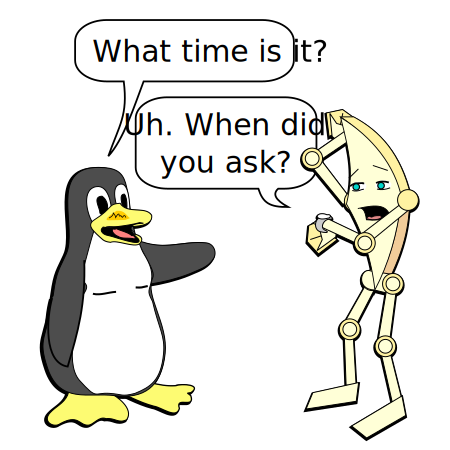
\includegraphics{cartoons/r-2014-What-time-is-it}}
\caption{What Time Is It?}
\ContributedBy{Figure}{fig:app:questions:What Time Is It?}{Melissa Broussard}
\end{figure}

A key issue with timekeeping on multicore computer systems is illustrated
by \cref{fig:app:questions:What Time Is It?}.
One problem is that it takes time to read out the time.
An instruction might read from a hardware clock, and might
have to go off-core (or worse yet, off-socket) to complete
this read operation.
It might also be necessary to do some computation on the value read out,
for example, to convert it to the desired format, to apply network time
protocol (NTP) adjustments, and so on.
So does the time eventually returned correspond to the beginning of
the resulting time interval, the end, or somewhere in between?

Worse yet, the thread reading the time might be interrupted or preempted.
Furthermore, there will likely be some computation between reading out
the time and the actual use of the time that has been read out.
Both of these possibilities further extend the interval of uncertainty.

One approach is to read the time twice, and take the arithmetic mean
of the two readings, perhaps one on each side of the operation being
timestamped.
The difference between the two readings is then a measure of uncertainty
of the time at which the intervening operation occurred.

Of course, in many cases, the exact time is not necessary.
For example, when printing the time for the benefit of a human user,
we can rely on slow human reflexes to render internal hardware and
software delays irrelevant.
Similarly, if a server needs to timestamp the response to a client, any
time between the reception of the request and the transmission of the
response will do equally well.

There is an old saying that those who have but one clock always
know the time, but those who have several clocks can never be sure.
And there was a time when the typical low-end computer's sole
software-visible clock was its program counter, but those days are
long gone.
This is not a bad thing, considering that on modern computer systems,
the program counter is a truly horrible
clock~\cite{PeterOkech2009InherentRandomness}.

In addition, different clocks provide different tradeoffs of performance,
accuracy, precision, and ordering.
For example, in the Linux kernel, the \co{jiffies} counter\footnote{
	The \co{jiffies} variable is a location in normal memory that
	is incremented by software in response to events such as the
	scheduling-clock interrupt.}
provides high-speed access to a course-grained counter (at best
one-millisecond accuracy and precision) that imposes very little ordering
on either the compiler or the hardware.
In contrast, the x86 HPET hardware provides an accurate and
precise clock, but at the price of slow access.
The x86 time-stamp counter (TSC) has a checkered past, but is more
recently held out as providing a good combination of precision, accuracy,
and performance.
Unfortunately, for all of these counters, ordering against all effects
of prior and subsequent code requires expensive memory-barrier instructions.
And this expense appears to be an unavoidable consequence of the
complex superscalar nature of modern computer systems.

\begin{figure}
\centering
\resizebox{3in}{!}{\includegraphics{CodeSamples/api-pthreads/QAfter/timeskewhist}}
\caption{\tco{clock_gettime(CLOCK_REALTIME)} Deviation From Immediately Preceding \tco{clock_gettime(CLOCK_MONOTONIC)}}
\label{fig:app:questions:clock-gettime(CLOCK-REALTIME) Deviation From Immediately Preceding clock-gettime(CLOCK-MONOTONIC)}
\end{figure}

In addition, each clock source provides its own timebase.
\Cref{fig:app:questions:clock-gettime(CLOCK-REALTIME) Deviation From Immediately Preceding clock-gettime(CLOCK-MONOTONIC)}
shows a histogram of the value returned by a call to
\co{clock_gettime(CLOCK_MONOTONIC)} subtracted from that returned by an
immediately following \co{clock_gettime(CLOCK_REALTIME)}
(\path{timeskew.c}).
Because some time passes between these two function calls, it is no
surprise that there are positive deviations, but the negative deviations
should give us some pause.
Nevertheless, such deviations are possible, if for no other reason than
the machinations of network time protocol (NTP).

Worse yet, identical clocksources on different systems
are not necessarily compatible with that of another.
For example, the \co{jiffies} counters on a pair of systems very likely
started counting at different times, and worse yet might well be counting
at different rates.
This brings up the topic of synchronizing a given system's counters
with some real-world notion of time such as the aforementioned NTP,
but that topic is beyond the scope of this book.

In short, time is a slippery topic that causes untold confusion to
parallel programmers and to their code.
